\documentclass[10pt, a5paper]{article}
\usepackage{pdfpages}
\usepackage{parallel}
\usepackage[T2A]{fontenc}
\usepackage{ucs}
\usepackage[utf8x]{inputenc}
\usepackage[polish,english,russian]{babel}
\usepackage{hyperref}
\usepackage{rotating}
\usepackage[inner=2cm,top=1.8cm,outer=2cm,bottom=2.3cm,nohead]{geometry}
\usepackage{listings}
\usepackage{graphicx}
\usepackage{wrapfig}
\usepackage{longtable}
\usepackage{indentfirst}
\usepackage{array}
\newcolumntype{P}[1]{>{\raggedright\arraybackslash}p{#1}}
\frenchspacing
\usepackage{fixltx2e} %text sub- and superscripts
\usepackage{icomma} % коскі ў матэматычным рэжыме
\PreloadUnicodePage{4}

\newcommand{\longpage}{\enlargethispage{\baselineskip}}
\newcommand{\shortpage}{\enlargethispage{-\baselineskip}}

\def\switchlang#1{\expandafter\csname switchlang#1\endcsname}
\def\switchlangbe{
\let\saverefname=\refname%
\def\refname{Літаратура}%
\def\figurename{Іл.}%
}
\def\switchlangen{
\let\saverefname=\refname%
\def\refname{References}%
\def\figurename{Fig.}%
}
\def\switchlangru{
\let\saverefname=\refname%
\let\savefigurename=\figurename%
\def\refname{Литература}%
\def\figurename{Рис.}%
}

\hyphenation{admi-ni-stra-tive}
\hyphenation{ex-pe-ri-ence}
\hyphenation{fle-xi-bi-li-ty}
\hyphenation{Py-thon}
\hyphenation{ma-the-ma-ti-cal}
\hyphenation{re-ported}
\hyphenation{imp-le-menta-tions}
\hyphenation{pro-vides}
\hyphenation{en-gi-neering}
\hyphenation{com-pa-ti-bi-li-ty}
\hyphenation{im-pos-sible}
\hyphenation{desk-top}
\hyphenation{elec-tro-nic}
\hyphenation{com-pa-ny}
\hyphenation{de-ve-lop-ment}
\hyphenation{de-ve-loping}
\hyphenation{de-ve-lop}
\hyphenation{da-ta-ba-se}
\hyphenation{plat-forms}
\hyphenation{or-ga-ni-za-tion}
\hyphenation{pro-gramming}
\hyphenation{in-stru-ments}
\hyphenation{Li-nux}
\hyphenation{sour-ce}
\hyphenation{en-vi-ron-ment}
\hyphenation{Te-le-pathy}
\hyphenation{Li-nux-ov-ka}
\hyphenation{Open-BSD}
\hyphenation{Free-BSD}
\hyphenation{men-ti-on-ed}
\hyphenation{app-li-ca-tion}

\def\progref!#1!{\texttt{#1}}
\renewcommand{\arraystretch}{2} %Іначай формулы ў матрыцы зліпаюцца з лініямі
\usepackage{array}

\def\interview #1 (#2), #3, #4, #5\par{

\section[#1, #3, #4]{#1 -- #3, #4}
\def\qname{LVEE}
\def\aname{#1}
\def\q ##1\par{{\noindent \bf \qname: ##1 }\par}
\def\a{{\noindent \bf \aname: } \def\qname{L}\def\aname{#2}}
}

\def\interview* #1 (#2), #3, #4, #5\par{

\section*{#1\\{\small\rm #3, #4. #5}}

\def\qname{LVEE}
\def\aname{#1}
\def\q ##1\par{{\noindent \bf \qname: ##1 }\par}
\def\a{{\noindent \bf \aname: } \def\qname{L}\def\aname{#2}}
}

\switchlang{ru}
\begin{document}
\title{Hubzilla --- введение, возможности, Hubzilla-сообщество \footnote{\url{tech@sprechrun.de} \url{http://lvee.org/ru/abstracts/244}}}
\author{Gustav Wall, Oldenburg(Oldb), Germany}
\maketitle
\begin{abstract}
Hubzilla is a free and open source platform running on a special kind of web server, called a <<hub>>, that can connect to other hubs in a decentralised network called <<the grid>>, providing sophisticated communications, identity, and access control services which work together seamlessly across domains and independent websites. It allows anybody to publicly or privately publish content via <<channels>>.
\end{abstract}
\subsection*{Что такое Хабзилла?}

\begin{center}
\begin{figure}[h!]
  \centering
  
\includegraphics[width=6cm]{Wall1.png}
  
  \label{Wall_1}
\end{figure}
\end{center}

Hubzilla (Хабзилла, в дальнейшем Hbz) ~--- это платформа в форме децентральной сети, созданная с целью обеспечить возможность общения без цензуры и с соблюдением приватности. Сама структура Hubzilla сети и Hbz протокол Zot \footnote{\url{https://hub.libranet.de/help/developer/zot_protocol}} обеспечивают комфортное общение всех участников сети на равных. Hubzilla обладает многими полезными свойствами. Важность, значение каждого из этих свойств в каждом конкретном случае зависит от того, для каких целей вы используете это платформу.

\subsection*{Свойства, важные для всех ~--- вездесущность и доступность}

Два замечательных свойства Hbz понятны, важны и привлекательны для всех пользователей этой платформы ~--- вездесущность и доступность.

\textbf{вездесущность} в контексте Hbz это:

\begin{itemize}
  \item с одной стороны \emph{вездесущность в буквальном глобальном \linebreak смысле}, т.е. способность и возможность для участников сети \linebreak Hubzilla получить доступ и пользоваться сервисами этой сети везде, где участник или участница сети имеют возможность войти в свою учётную запись и контактировать своего виртуального \emph{кочующего двойника}. Неисправность одного из узлов не оказывает существенного влияния ни на работоспособность отдельных участников сети, ни на работоспособность сети в целом.
  \item вездесущность в смысле возможности \emph{с небольшими затратами времени обменивать сообщения с большим \linebreak количеством контактов}. Эта вездесущность обеспечивается за счёт того, что при вводе сообщения участники Hbz-сети простым вводом символа \textbf{@(собака)} с последующим вводом какой-нибудь буквы или нескольких букв могут показать \textbf{все контакты}, содержащие введённую последовательность символов. Такой контакт может быть и рассылкой. Каждый подписчик рассылки может получить сообщение без того, что отправитель и получатель до этого общались.
\end{itemize}

Необычно \textbf{высокие значения доступности сервисов} в смысле ITIL \footnote{\url{https://itsm365.ru/blog/upravlenie-dostupnostyu-availability-}\linebreak \url{management-po-itil/}} являются ещё одним уникальным свойством Hbz сети и достигается благодаря вездесущности его участников. Доступность самой сети и вездесущность её участников ~--- это две стороны одной медали. В сети Hbz доступность, стабильность сети растёт пропорционально с увеличением количества её участников.

\subsection*{Кочующий двойник и другие удобства}

\textbf{Кочующий двойник} является одним из центральных понятий в Hbz-сети, которое позволяет реализовать в сети эффект вездесущности. Уникальное свойство  вездесущности возможно благодаря тому, что участники могут на своё усмотрение с согласия оператора узла размещать свою учётную запись параллельно на разных узлах сети, удалять эту запись, что приводит к \textbf{повышению надёжности доступа к учётной записи практически до 100\%}. Если участник изменит данные на одном из узлов, обновляются данные и на узлах-двойниках. Непрерывно в режиме реального времени двойники обменивают данные, благодаря чему любой из двойников постоянно знает то, что знает и его протагонист.

\subsection*{Доступно по умолчанию}

Следующими возможностями могут пользоваться владельцы узла после установки Hbz \textbf{по умолчанию}:

\begin{itemize}
  \item адресная книга (контакты)
  \item сайт, веб-ресурс
  \item социальные сети
  \item форумы
  \item календарь мероприятий
  \item вики
  \item чат
  \item облачное хранилище файлов
  \item набор приложений (apps), который может расширяться в соответствии с потребностями владельца узла.
\end{itemize}

Обмен сообщениями в сети производится в соответствии с https-протоколом. Дополнительно имеется возможность закодировать \linebreak часть или всё сообщение паролем.

\subsection*{Многосторонне одарённый двойник}

\textbf{Общительность} --- способность обменивать сообщения с другими сетями, например такими как Диаспора\footnote{\url{https://ru.wikipedia.org/wiki/Diaspora}} или Фриндика\footnote{\url{https://ru.wikipedia.org/wiki/Friendica}}.

\textbf{Всеядность} ~--- способность переваривать, интегрировать множество форматов ~--- \emph{HTML}, простой текст, \emph{bbcode, markdown, \linebreak application/x-php}, благодаря чему пользователи могут в своих сообщениях комбинировать содержимое из разных источников с малыми затратами времени.

\textbf{Универсальность, неприхотливость} ~--- в зависимости от нагрузки на конкретном узле Hbz, зависящей от количества зарегистрированных пользователей, от активности, в том числе от количества контактов этих пользователей и от количества посетителей на узле можно установить этот узел на соответствующем железе ~--- Hbz работает на мини-компьютере Raspberry Pi \footnote{\url{https://www.raspberrypi.org/}} так же надёжно, как на сервере с мощнейшими AMD- или Intel-Xeon- мультипроцессорами.

\subsection*{Виртуальный кабинет ~--- рабочее место двойника}

Zot ~--- это \footnote{\url{https://hub.libranet.de/help/developer/zot_protocol}} специальный протокол, который обеспечивает обмен информацией, управление двойниками и управление доступом в децентральной сети, состоящей из независимых узлов (hubs). Эту сеть в Hbz-контексте часто называют грид (grid). Hbz-узлы выполняют различные функции, важнейшие из которых для владельца узла:

\begin{itemize}
  \item предоставление \textbf{виртуального кабинета} \emph{кочующему двойнику} владельца узла, который имеет в своём распоряжении:
  \begin{itemize}
	  \item контакты владельца узла
	  \item место встречи с другими двойниками
	  \item своего рода \textbf{передающую станцию} с одним или множеством каналов или \textbf{издательство} с одним или множеством изданий
	  \item систему для \textbf{прецизионного управления доступом} к каждому из объектов на узле
  \end{itemize}
  \item двойник в соответствии с доверенными ему полномочиями выполняет массу дел, связанных с общением с другими двойниками из сети Hbz или с гостями сети
  \item практически неограниченное количество принадлежащих владельцу узла \textbf{виртуальных кабинетов}, куда он может пустить как \emph{постояльцев} чужих двойников:
	\begin{itemize}
	  	\item каждый из чужих двойников имеет в своём распоряжении практически те же возможности, что двойник владельца узла, особенно если постоялец и владелец доверяют друг другу или они заключили соответствующий договор о найме виртуального кабинета.
	\end{itemize}
\end{itemize}

Таким образом сеть Hbz представляет собой пространство, среду обитания для двойников, объём полномочий которых предопределяется оригиналом.

\subsection*{Возможности применения}

Картинки отображают образно или схематично возможные сценарии применения Hbz. MicroSD отображает тот факт, что сервер Hubzilla можно установить на этой карте размером с ноготок.

\begin{center}
\begin{figure}[h!]
  \centering
  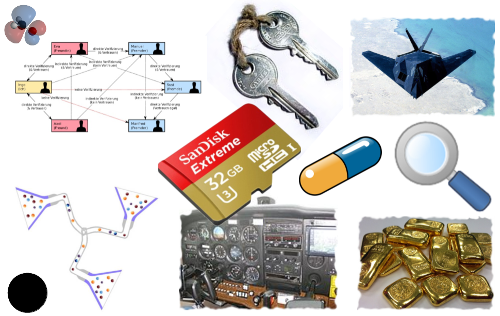
\includegraphics[width=6cm]{Wall2.png}
  
  \label{Wall2}
\end{figure}
\end{center} 

\begin{thebibliography}{20}
\bibitem{Wall-1} Hubzilla помощь ~--- \url{http://hub2.sprechrun.de/help/}
\bibitem{Wall-2} The history of Hubzilla ~--- \url{http://www.talkplus.org/blog/2016/the-history-of-hubzilla/}
\bibitem{Wall-3} Аккаунт, двойник автора (Gustav Wall) в сети Хабзилла ~--- \url{https://\%hub.libranet.de/channel/nmoplus}
\bibitem{Wall-4} Web of Trust Von \url{https://commons.wikimedia.org/wiki/User/Ogmios} ~--- \url{https://upload.wikimedia.org/wikipedia/commons} ~--- \url{https://upload.wikimedia.org/wikipedia/commons/4/4e/Web\_of\_Trust.svg, CC BY-SA 3.0}, \url{https://commons.wikimedia.org/w/index.php?curid=30127548}
\bibitem{Wall-5} Zwei gleiche Schlüssel Von Sebastian Hartlaub ~--- Eigenes Werk, CC BY-SA 3.0, \url{https://commons.wikimedia.org/w/index.php?curid=696513}
\end{thebibliography} 

\end{document}
